%\documentclass[a4paper,12pt,english,twoside,openright]{book}
\documentclass[english,12pt,booktabs,hyperref,titling,twoside,openright]{hepthesis}
%%% hepthesis requirements
\usepackage{setspace,fancyhdr,rotating,comment,tocbibind,changepage,varwidth,csquotes,babel,a4wide,amsmath,hyperref,booktabs,draftcopy,lineno}
%\usepackage[babel]{csquotes}
\usepackage{hepnames,hepunits,hepparticles}
\usepackage{epsfig,amssymb,latexsym,numprint,textcomp}
%\usepackage[utf8]{inputenc}
%\usepackage{appendix}
%\usepackage{epstopdf}
\usepackage{subfigure}
\usepackage{graphicx}
\usepackage{color}
\usepackage[backend=biber, sorting=none]{biblatex}
\usepackage[format=plain,labelfont=bf]{caption}
\usepackage{enumerate}
\usepackage{lscape}
\usepackage{emptypage}
\usepackage{pifont}
\usepackage{multirow}

\graphicspath{/home/lviliani/Documenti/PhdThesis/images}
\let\oldGeV\GeV
\let\oldTeV\TeV
\renewcommand{\GeV}{\,\oldGeV \xspace}
\renewcommand{\TeV}{\,\oldTeV \xspace}
\newcommand{\hww}{\ensuremath{{\mathrm{H}\to\mathrm{WW}}}\xspace}
\newcommand{\hwwllnn}{\ensuremath{{\mathrm{H}\to\mathrm{WW}\to\mathrm{2\ell2\nu}}}\xspace}
\newcommand{\ttH}{\ensuremath{\mathrm{t\bar{t}H}}\xspace}
\newcommand{\fb}{\ensuremath{\mathrm{fb}}\xspace}
\newcommand{\pb}{\ensuremath{\mathrm{pb}}\xspace}
\newcommand{\ifb}{\ensuremath{\mathrm{fb^{-1}}}\xspace}
\newcommand{\ipb}{\ensuremath{\mathrm{pb^{-1}}}\xspace}
\newcommand{\WW}{\ensuremath{\mathrm{WW}}\xspace}
\newcommand{\W}{\ensuremath{\mathrm{W}}\xspace}
\newcommand{\F}{\ensuremath{\cmsSymbolFace{F}}}
\newcommand{\V}{\ensuremath{\cmsSymbolFace{V}}\xspace}
\newcommand{\VVV}{\cmsSymbolFace{VVV}\xspace}
\newcommand{\Wjets}{\ensuremath{\PW\text{+jets}}\xspace}
\newcommand{\X}{\ensuremath{\cmsSymbolFace{X}}\xspace}
\newcommand{\delphill}{\ensuremath{\Delta\phi_{\ell\ell}}}
\newcommand{\delphillmet}{\ensuremath{\Delta\phi(\ell\ell,\VEtmiss)}}
\newcommand{\dyll}{\ensuremath{Z/\gamma^*\to \ell^+\ell^-}\xspace}
\newcommand{\dymm}{\ensuremath{Z/\gamma^*\to\Pgmp\Pgmm}}
\newcommand{\dytt}{\ensuremath{Z/\gamma^* \to\tau^+\tau^-}}
\newcommand{\jp}{\ensuremath{J^{P}}\xspace}
\newcommand{\mll}{\ensuremath{m_{\ell\ell}}\xspace}
\newcommand{\mt}{\ensuremath{m_\mathrm{T}}\xspace}
\newcommand{\psvectorKD}{\ensuremath{\mathcal{D}_{1^-}}\xspace}
\newcommand{\ptl}{\ensuremath{p_\perp^{\ell}}\xspace}
\newcommand{\ptll}{\ensuremath{\pt^{\ell\ell}}\xspace}
\newcommand{\MET}{\ensuremath{E_\mathrm{T}^\mathrm{\,miss}}\xspace}
\newcommand{\ptmiss}{\ensuremath{\vec{p}_\mathrm{T}^\mathrm{\,miss}}\xspace}
\newcommand{\qq}{\ensuremath{\Pq\Pq}\xspace}
\newcommand{\superKD}{\ensuremath{\mathcal{D}_\text{bkg}} }
\newcommand{\tw}{\ensuremath{\cPqt\PW}\xspace}
\newcommand{\vectorKD}{\ensuremath{\mathcal{D}_{1^+}} }
\newcommand{\wgamma}{\ensuremath{\PW\gamma}\xspace}
\newcommand{\mjj}{\ensuremath{m_{jj}}\xspace}
\newcommand{\pt}{\ensuremath{p_\mathrm{T}}\xspace}
\newcommand{\pth}{\ensuremath{p_\mathrm{T}^\mathrm{H}}\xspace}
\newcommand{\ttbar}{\ensuremath{\mathrm{t}\bar{\mathrm{t}}}\xspace}
\newcommand{\jpb}{{\em JetBProbability }\xspace}
\newcommand{\tg}{{\em tag}\xspace}
\newcommand{\probe}{{\em probe}\xspace}
\newcommand{\tp}{{\em tag-probe}\xspace}
\newcommand{\tpp}{{\em tag-pass-probe}\xspace}
\newcommand{\tfp}{{\em tag-fail-probe}\xspace}


\pdfinfo{%
  /Title    (PhD Thesis)
  /Author   (Lorenzo Viliani)
}


\bibliography{PhDThesis}

\begin{document}

\begin{frontmatter}

\title{Measurement of the Higgs boson transverse momentum spectrum in the WW decay channel at 8\,TeV and first results at 13\,TeV}
\author{Lorenzo Viliani}

\titlepage[of University of Florence]{PhD Thesis}

\begin{abstract}
The cross section for Higgs boson production in pp collisions is studied using the $\mathrm{H} \to \mathrm{W}^+ \mathrm{W}^-$  decay mode, followed by leptonic decays of the W bosons, leading to an oppositely charged electron-muon pair in the final state. 
The measurements are performed using data collected by the CMS experiment at the LHC with pp collisions at a centre-of-mass energy of 8\TeV, corresponding to an integrated luminosity of 19.4\ifb.
The Higgs boson transverse momentum (\pt) is reconstructed using the lepton pair \pt and missing \pt. The differential cross section times branching fraction is measured as a function of the Higgs boson \pt in a fiducial phase space defined to match the experimental acceptance in terms of the lepton kinematics and event topology. The production cross section times branching fraction in the fiducial phase space is measured to be $39 \pm 8~$(stat)$~\pm 9~$(syst)\fb. The measurements are compared to theoretical calculations based on the standard model to which they agree within experimental uncertainties.
\end{abstract}

%\pagestyle{empty}
\cleardoublepage
%\pagenumbering{roman}
\pagestyle{fancy}
\fancyhead{}
\fancyfoot{}
\fancyhead[RO]{\thepage}
\fancyhead[LE]{\thepage}
\tableofcontents
\cleardoublepage

\end{frontmatter}

\begin{mainmatter}

\input Chapter1/chapter1.tex
\input Chapter2/chapter2.tex
\input Chapter3/chapter3.tex
\input Chapter4/chapter4.tex
\input Chapter5/chapter5.tex
\input Chapter6/chapter6.tex
\clearpage
\appendix
\chapter{Fiducial phase space definition and optimization}\label{app:fiducial_region}
\markboth{Fiducial phase space definition and optimization}{Fiducial phase space definition and optimization}
\thispagestyle{empty}
	
The generator level fiducial phase space definition must be chosen to closely match the selections applied in the analysis at the reconstructed level, in order to reduce the model dependence in the extrapolation step. This means that, for optimizing the fiducial phase space definition, the efficiency $\varepsilon_\mathrm{fid}$ (see Sec.~\ref{sec:fid_space}) has to be maximized. Another parameter playing an important role is the fraction of out-of-fiducial signal events (also called fakes), $f_\text{out-of-fid}$, that is the number of reconstructed events generated by the signal process that do not belong to the fiducial phase space. This parameter should instead be as small as possible. A simplistic way to improve the fiducial phase space definition is to maximize the ratio between the overall efficiency and out-of-fiducial rate.

Several different fiducial region definitions have been tested and the results show that:
\begin{itemize}
\item {\bf Leptons flavour:} the fiducial phase space definition must include only the opposite flavour combination including one electron and one muon. If the combinations involving $\tau$ leptons are included the efficiency falls down;
\item {\bf Leptons selections:} given the good resolution on lepton transverse momentum, there is no need to loosen the cuts related to these variables, i.e. the same cuts defined in the analysis selection can be kept also at generator level;
\item {\bf Neutrino pair \boldmath$\pt$ cut:} since the resolution on the measurement of the missing transverse energy is poor, the neutrino pair cut should not be included in the definition of the fiducial region, because it would increase the fake rate without increasing the efficiency, thus resulting in a lower ratio between overall efficiency and out-of-fiducial rate;
\item {\bf \boldmath$\mt$ cut:} also, the \mt cut in the analysis selection, i.e. $\mt>60$\GeV, must be loosened because it involves neutrinos, therefore increasing the fraction of out-of-fiducial events. This cut has been loosened to 50\GeV at generator level.
\end{itemize}

\begin{comment}
The fake rate and the efficiency as a function of \pth after the optimization discussed before are shown in figure \ref{fig:eff_fake_comp}. To obtain these plots the fiducial region was modified adding in sequence the various cuts and computing the efficiency and the fake rate each time. In that way we can asses the composition of those distributions.

\begin{figure}[htb]
\centering
\subfigure{
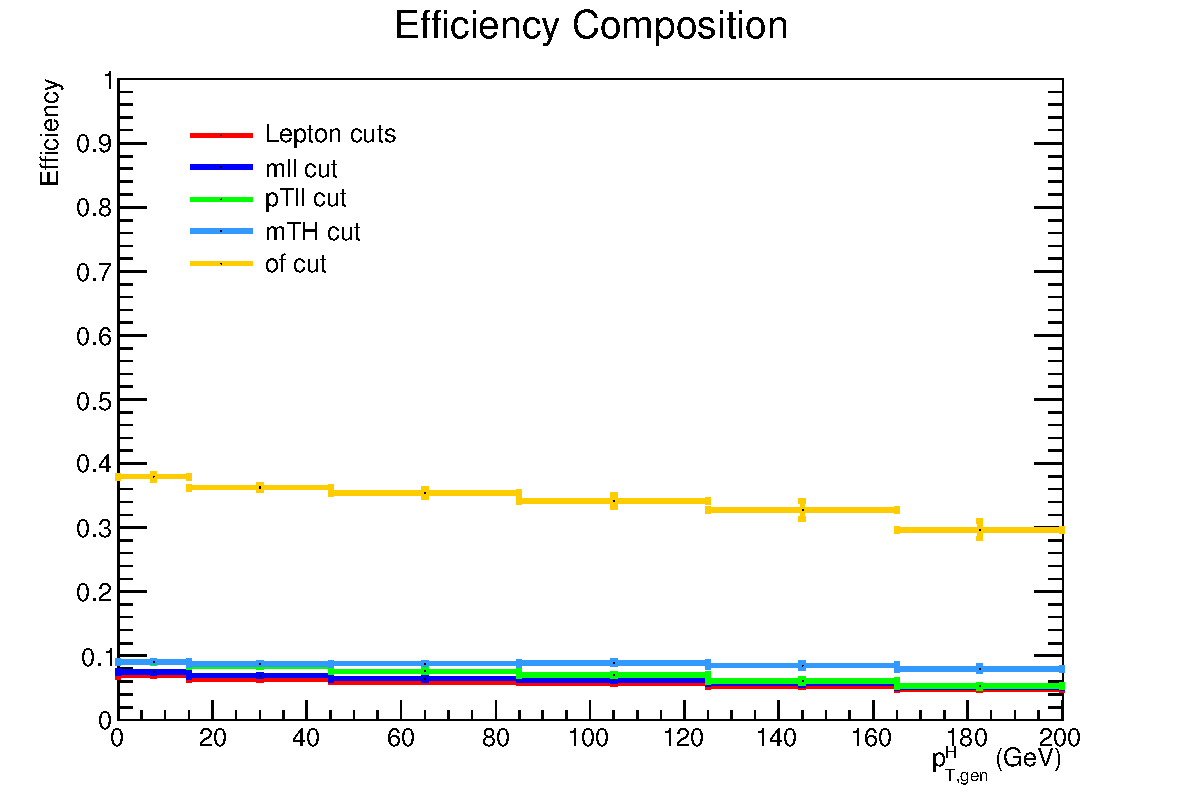
\includegraphics[width=0.5\textwidth]{images/eff_optimized.pdf}
}
\subfigure{
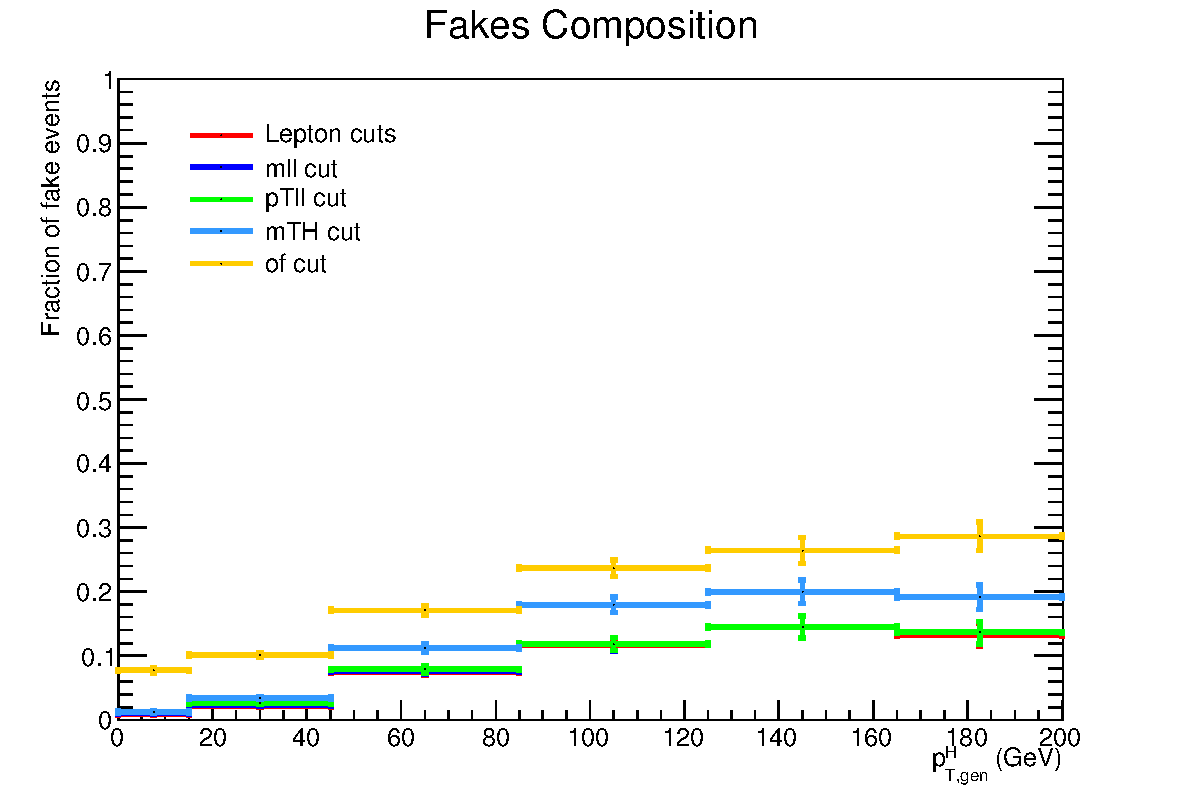
\includegraphics[width=0.5\textwidth]{images/fake_optimized.pdf}
}
\caption{Efficiency and fake rate as a function on Higgs transverse momentum. The plots correspond to the optimized fiducial region definition and show the effect of adding each of the mentioned cuts in sequence.}\label{fig:eff_fake_comp}
\end{figure}
\end{comment}
The efficiency and fraction of fake events have been measured also as a function of the \MET and \mt cuts in the fiducial phase space. Since these two variables are correlated, the results are reported as two-dimensional histograms. In Fig.~\ref{fig:eff_fake_nom} the efficiency and fraction of out-of-fiducial events for these two variables are reported.

\begin{figure}[htb]
\centering
\subfigure{
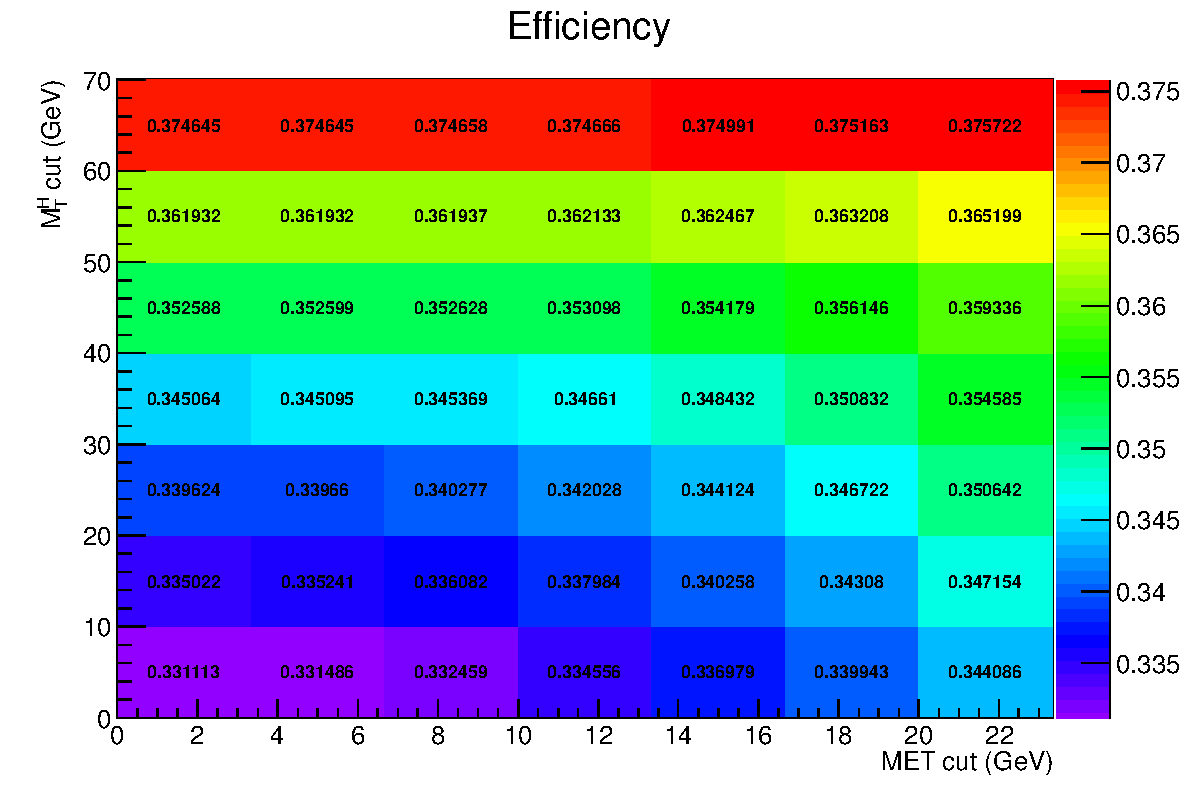
\includegraphics[width=0.4\textwidth]{images/met_mth_eff.pdf}
}
\subfigure{
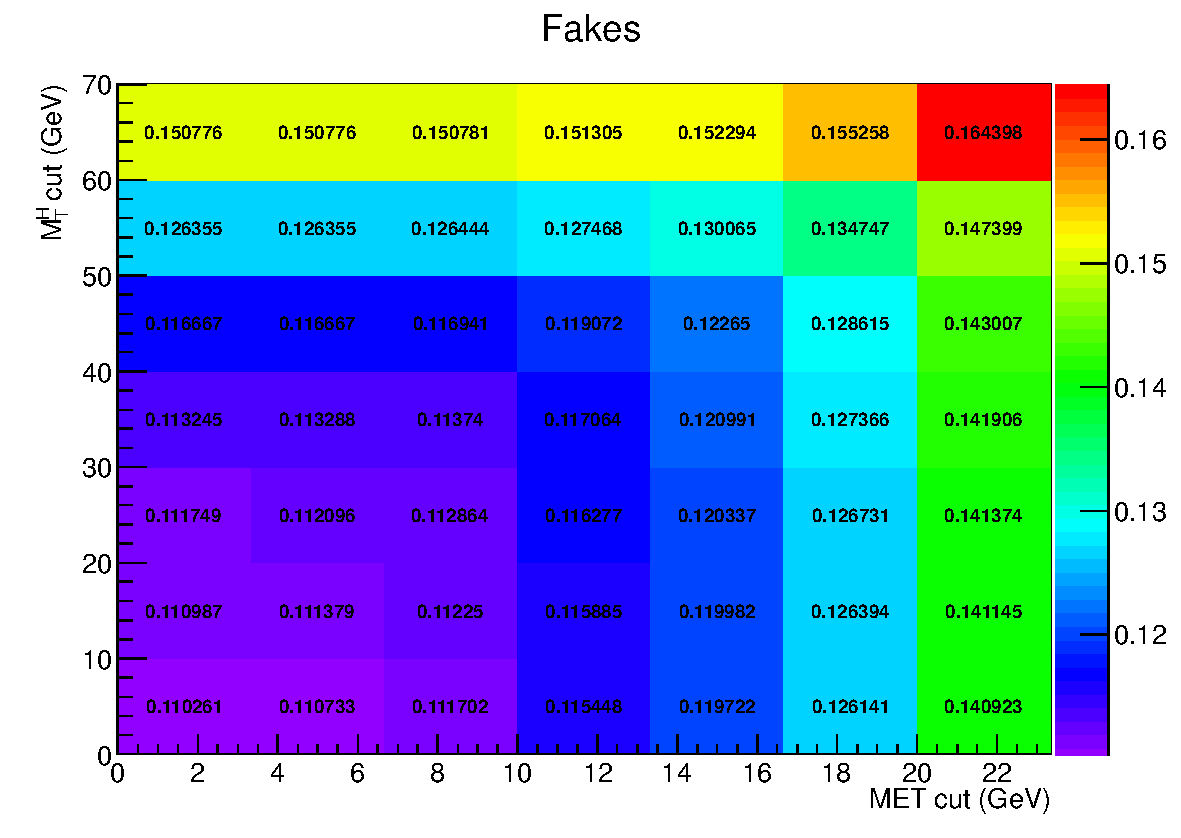
\includegraphics[width=0.4\textwidth]{images/met_mth_fake.pdf}
}
\caption{Efficiency and out-of-fiducial rate as a function of \MET and \mt cuts in the fiducial phase space.}\label{fig:eff_fake_nom}
\end{figure}

The criterion adopted to define the fiducial phase space is a trade-off between having large efficiency and small fraction of fake events. Especially when looking at the low resolution variables, such as \MET and \mt, a suitable figure of merit has to be chosen for the estimation of the best cuts. Several different figures of merit have been checked, such as $\varepsilon_\mathrm{fid}/f_\text{out-of-fid}$, $\varepsilon_\mathrm{fid} - f_\text{out-of-fid}$ and $(1-f_\text{out-of-fid})/\varepsilon_\mathrm{fid}$. The results for these three different figures of merit are shown in Fig.~\ref{fig:fig_merit_nom} as a function of the \MET and \mt cuts in the fiducial region. These three figures of merit have been used to establish the selections in the generator level fiducial phase space for the low resolution variables.

\begin{figure}[htb]
\centering
\subfigure{
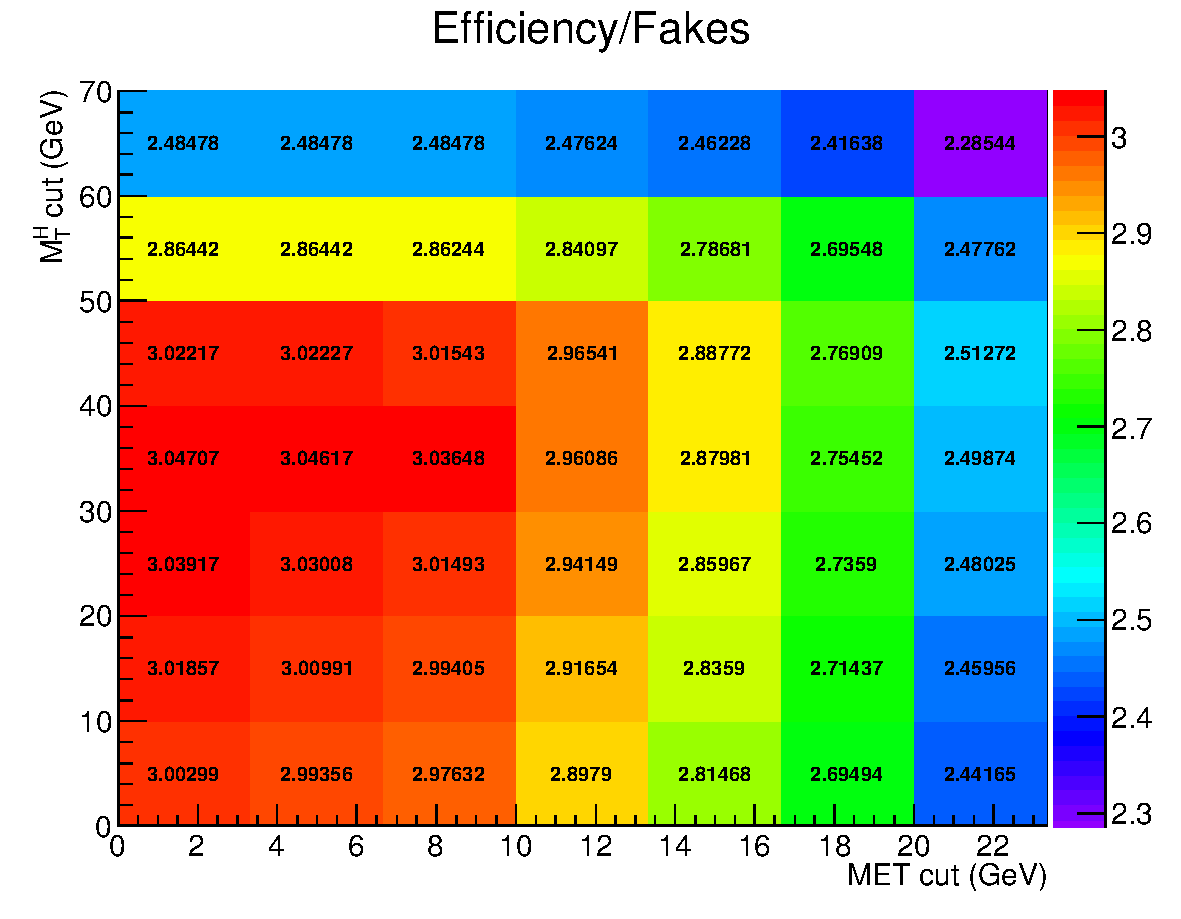
\includegraphics[width=0.4\textwidth]{images/eff_over_fake.pdf}
}
\subfigure{
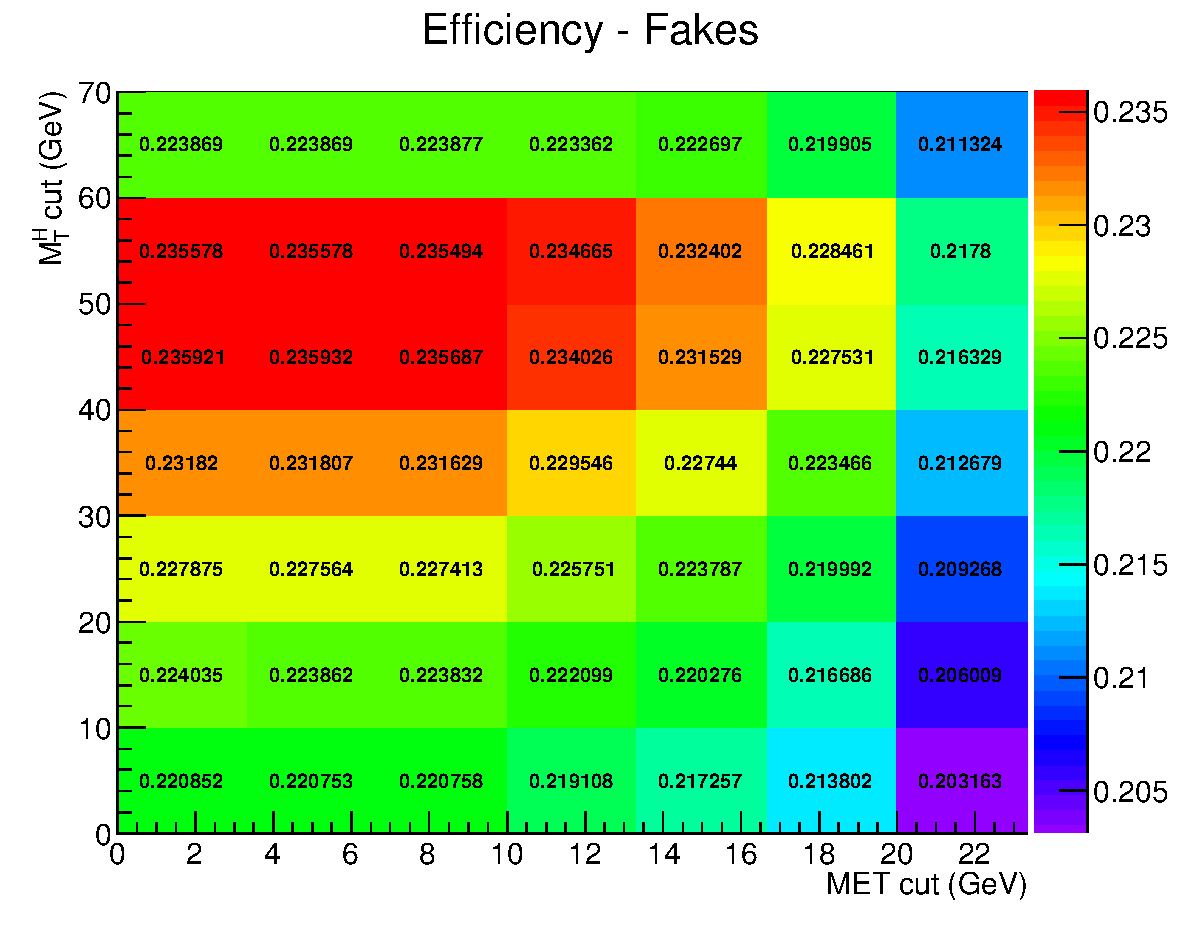
\includegraphics[width=0.4\textwidth]{images/eff-fakes.pdf}
}\\
\subfigure{
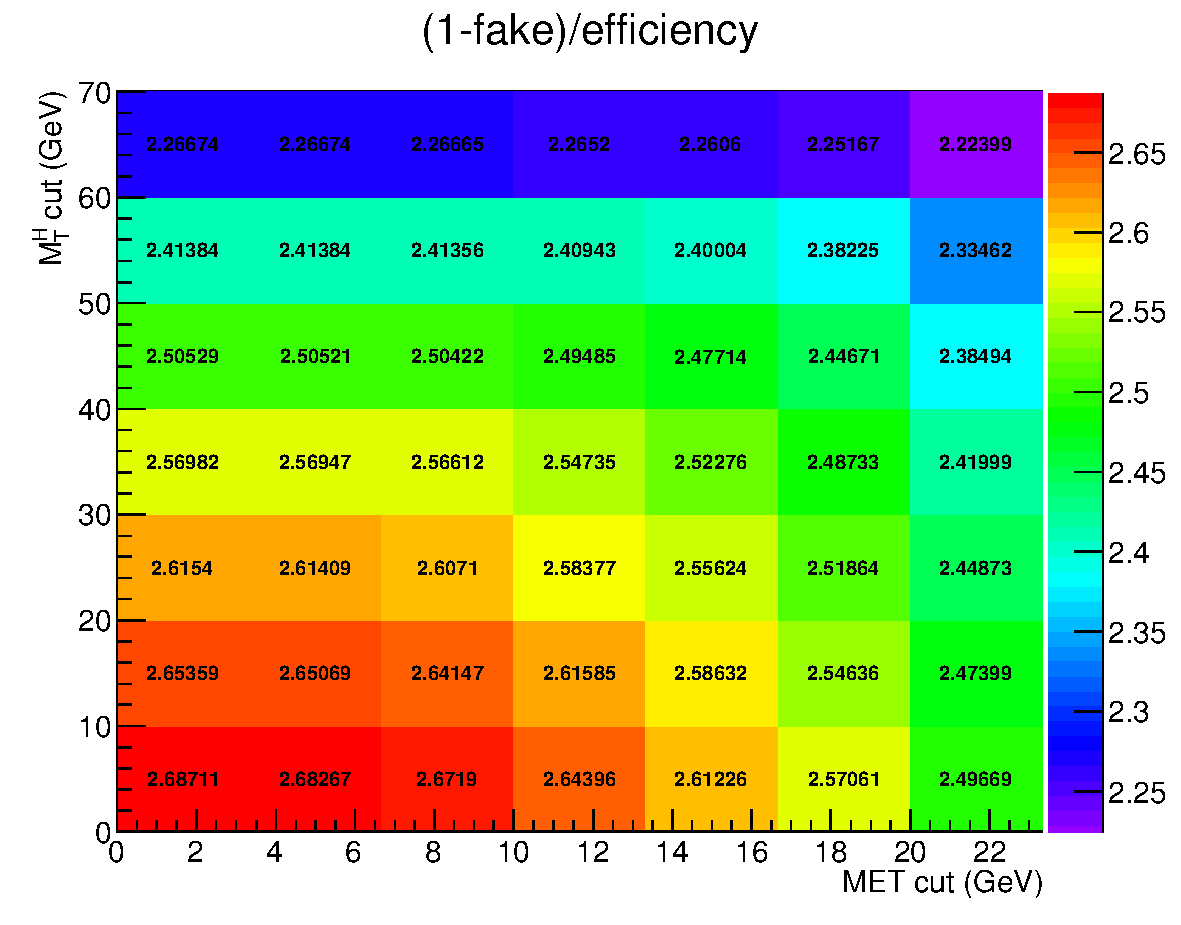
\includegraphics[width=0.4\textwidth]{images/1-fake_over_eff.pdf}
}
\caption{Different figures of merit as a function of \MET and \mt cuts in the fiducial phase space.}\label{fig:fig_merit_nom}
\end{figure}

\begin{comment}
Following the same criterion, similar plots as above have been obtained for an alternative model, given by varying up the ggH/VBF ratio within the experimental uncertainties. The results, shown in Fig.~\ref{fig:eff_fake_up} and Fig.~\ref{fig:fig_merit_up}, show a similar trend with respect to the model with nominal ggH/VBF ratio.

\begin{figure}[htb]
\centering
\subfigure{
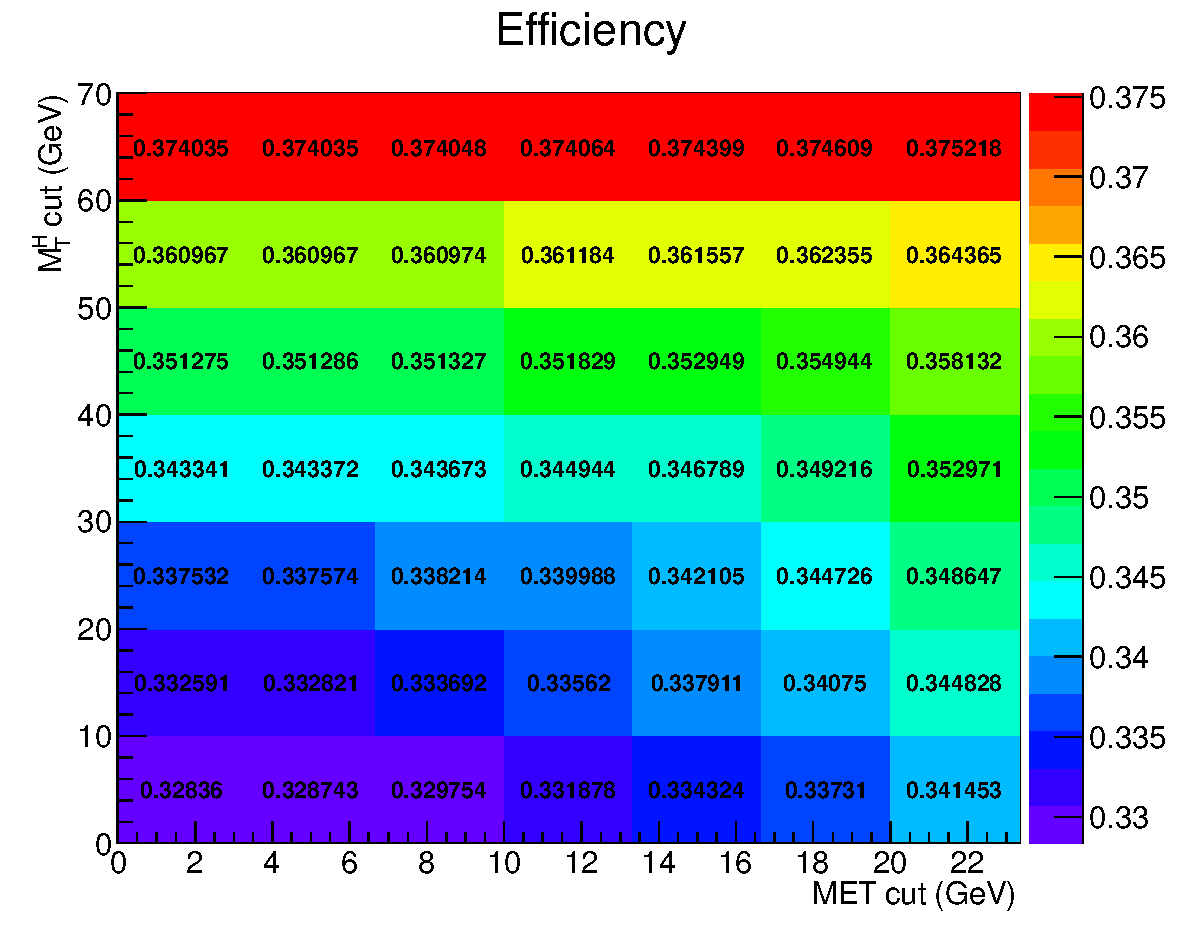
\includegraphics[width=0.4\textwidth]{images/met_mth_eff_UP.pdf}
}
\subfigure{
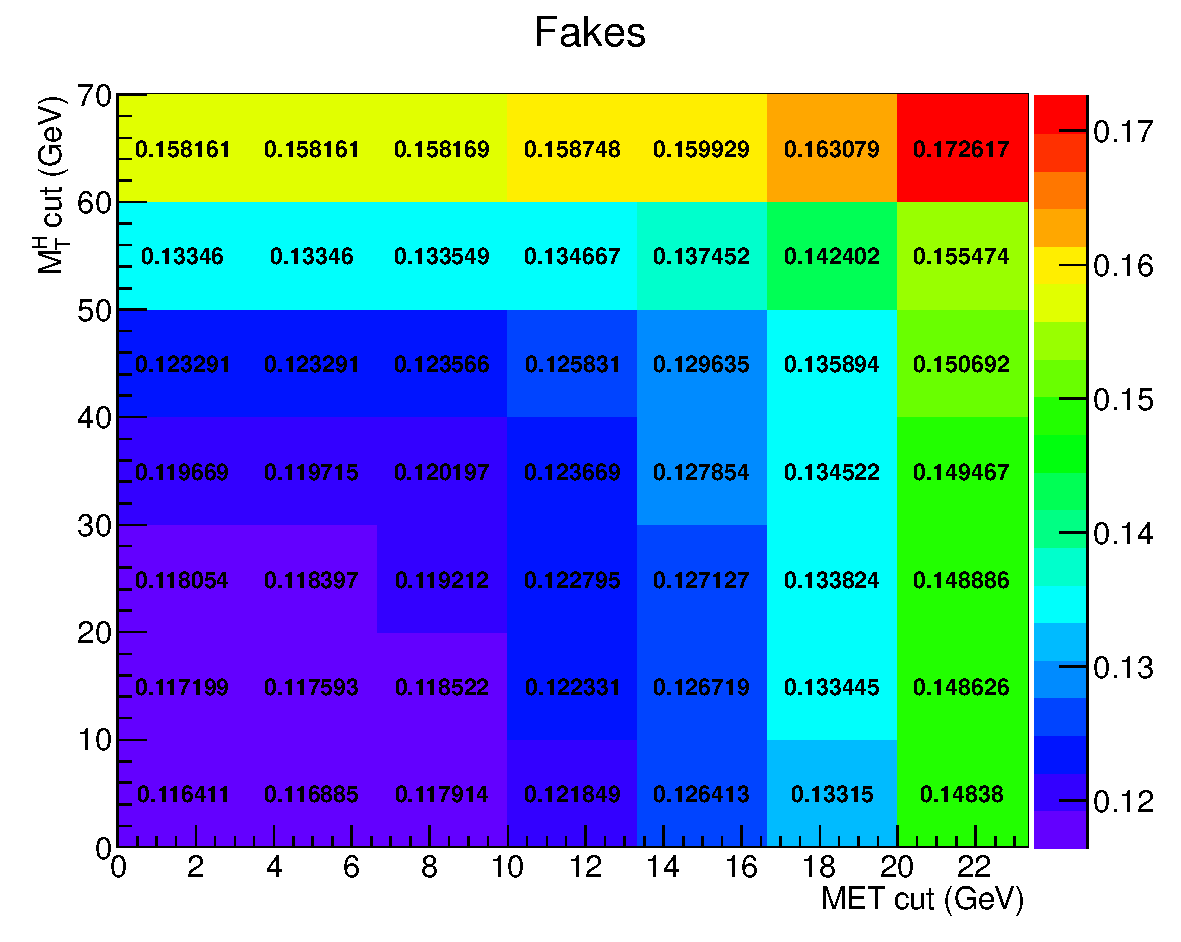
\includegraphics[width=0.4\textwidth]{images/met_mth_fake_UP.pdf}
}
\caption{Efficiency and out-of-fiducial rate as a function of \MET and \mt cuts in the fiducial region, for the alternative model with an up variation of the ggH/VBF ratio.}\label{fig:eff_fake_up}
\end{figure}

\begin{figure}[htb]
\centering
\subfigure{
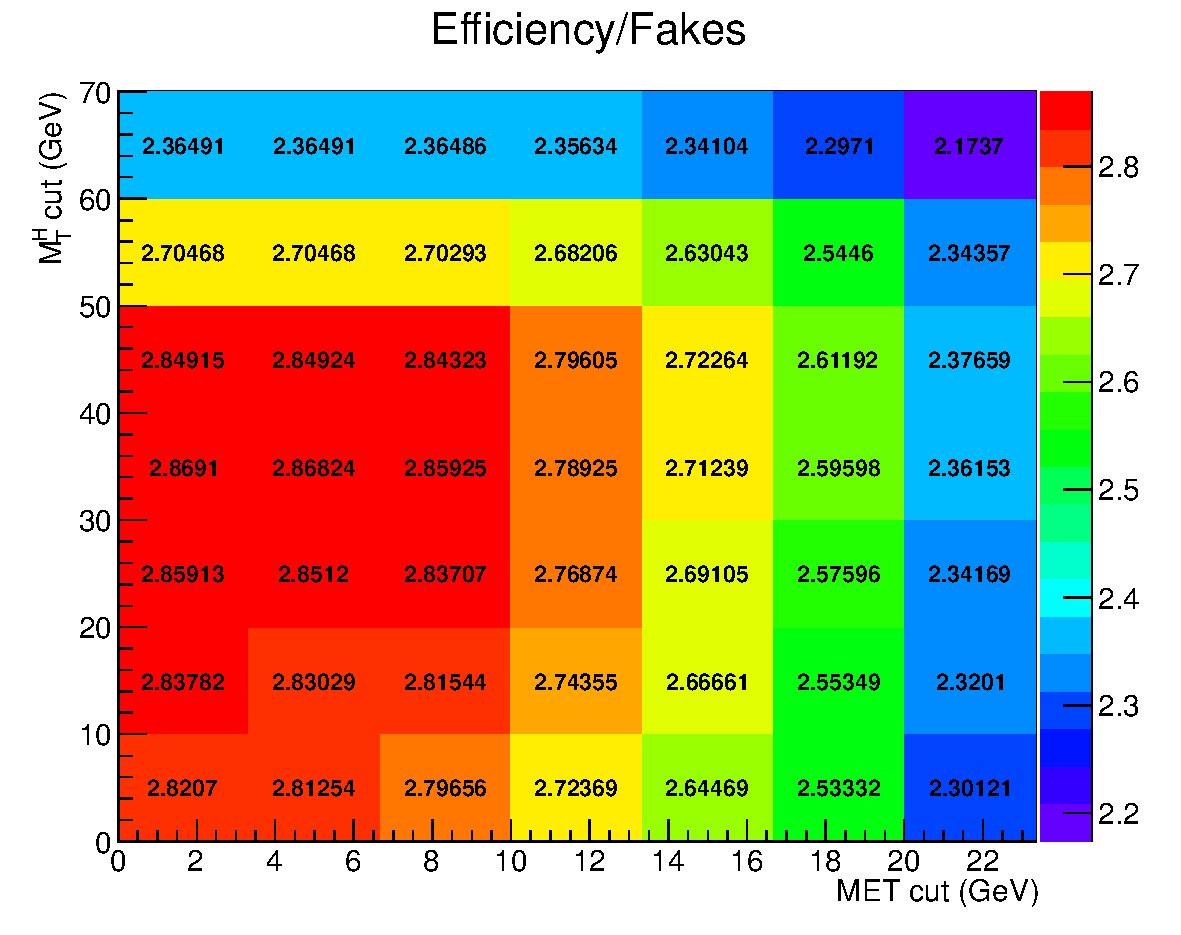
\includegraphics[width=0.5\textwidth]{images/eff_over_fake_UP.pdf}
}
\subfigure{
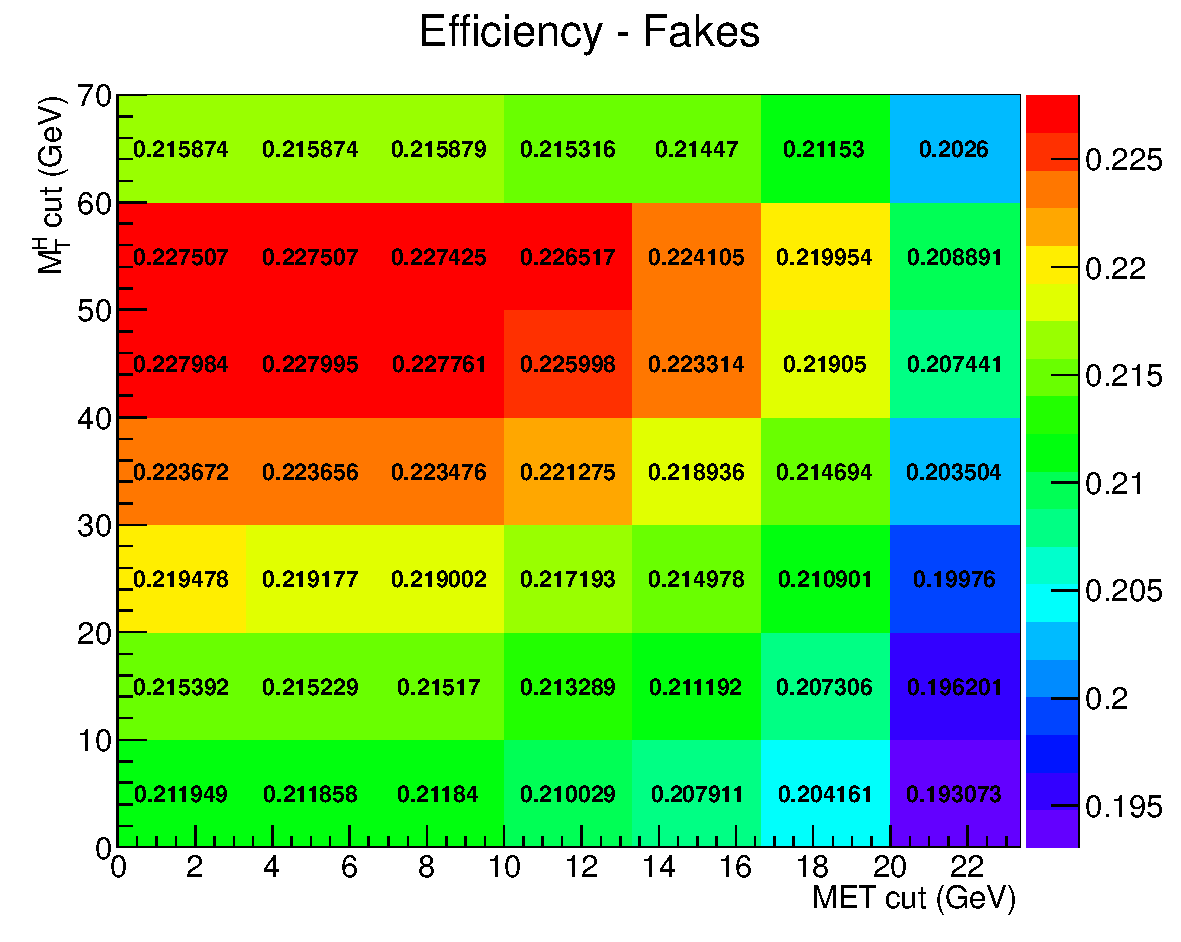
\includegraphics[width=0.5\textwidth]{images/eff-fakes_UP.pdf}
}\\
\subfigure{
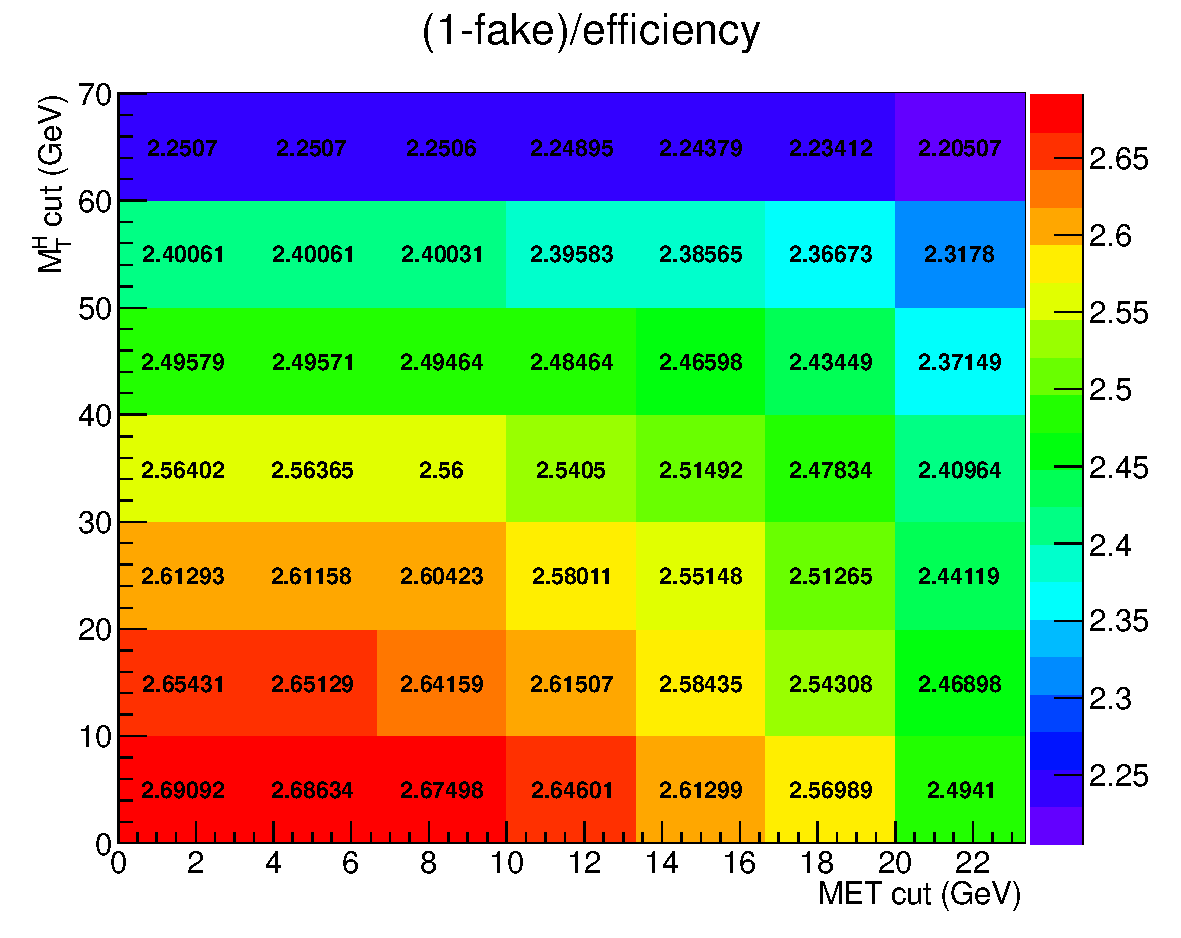
\includegraphics[width=0.5\textwidth]{images/1-fake_over_eff_UP.pdf}
}
\caption{Different figures of merit as a function of \MET and \mt cuts in the fiducial region, for the alternative model with an up variation of the ggH/VBF ratio.}\label{fig:fig_merit_up}
\end{figure}
\end{comment}

\end{mainmatter}

\begin{backmatter}

\clearpage\thispagestyle{empty}\cleardoublepage
\addcontentsline{toc}{section}{\bibname}
\printbibliography
\clearpage\thispagestyle{empty}\cleardoublepage
%\pagestyle{empty}

\end{backmatter}

\end{document}
